% Drawing 69/04-8 -- folder 69, batch 04, archive page 80 (PDF page 81).
% Transcription: en haut à gauche, un grand polyèdre en perspective aux sommets $u$, $v$, $w$ (triangle en trait épais), $u'$, $u''$, $v'$, $v''$, $w'$, $w''$, $\xi$, $\eta$, $e$, $f$ ; à côté du lemme, deux hexagones, un rectangle surmonté d'un triangle, un « U » fermé par un segment, une chaîne de segments marqués $(u,v)$, $(u',v')$, $(u,v'')$, $(u'',v)$, $(u',v')$, $(u',v)$. Au-dessous, plusieurs cubes et prismes aux sommets $u$, $v$, $u'$, $u''$, $v'$, $v''$, $w'$, $w''$, $\xi$, $\eta$ ; des octaèdres aux sommets $x$, $y$, $s$, $t$, $\xi$, $\eta$ ; un losange aux sommets $\alpha$, $\beta$, $\gamma$ ; un triangle aux sommets $\gamma_4$, $\beta'_4$, $\alpha_4$, $\gamma_1$ ; et, écrites en travers de la page, les listes $\beta_1\,\beta_2\,\beta_3\,\beta_4$, $\beta'_1\,\beta'_2\,\beta'_3\,\beta'_4$, $\gamma_1$, $\gamma_2$, $\gamma_4$, $\alpha_1$, $\alpha'_2$ et « $V\times V\times V$ ».
% Kind: page of polyhedra sketches (polyhedron uvw, hexagons, cubes, prisms, octahedra). Method 2 (schematic redraw from the facsimile). Status: partial.
% Notes: Whole page, each sketch redrawn at its place from tight crops, vertices placed once and every stroke drawn between them: the large polyhedron (top left) with the thick triangle u v w, the edges to w', w'', xi, eta and the lower ring u', u'', v', v'' (two faint inner diagonals); the left column, two prisms on u, v, u', v', u'', v'' (the second with w', w'' below); the middle column, a prism and a figure on xi, eta, u', v', u'', v'', w', w''; the U closed by a segment and the chain of segments marked (u,v), (u',v'), (u,v''), (u',v); the arrow; two hexagons; the rectangle with a triangle on it and an arrow inside; the octahedra x, y, s, t and xi, eta (their hidden axis dashed); the small triangle; an open figure; an open quadrilateral over a triangle (marked 3 and 5); the rhombus alpha beta gamma with its heavy fourth vertex; the figure gamma_4, beta'_4, alpha_4, with the small angle by gamma_1. Not drawn: a row of small dots marked u'', u', v', v'' in the middle of the page, the long diagonal strokes across the sheet, the lemma text, the lists written across the page and the lines towards e, f at the top. Still differs from the facsimile: the large polyhedron and the middle-column figure are overdrawn and given by their main strokes (which strokes are edges is a reading); the figure gamma_4, beta'_4, alpha_4 is drawn as its separate doubled strokes, which do not close on the page; most letters of the cubes and prisms are placed where they stand, others are left out. Redrawn 2026-11-09 (issue 128): vertices placed once and every edge drawn between them, labels at \small, strike-outs not drawn; to check again. Question settled by a machine pass on the facsimile, 2026-11-12 (page): the large polyhedron lacked the two outer vertices e and f named by the transcription: on the page each is joined by two long strokes to v' and v''; the two vertices, their letters and the four strokes are added. The rest of the page agrees with the overlay figure by figure; remaining differences are those listed above. Overlay check 2026-11-13 (claude-opus-5-5, issue 147): the 300 dpi colour rendering of the 250 ppi scan laid under the whole redraw, rasterised from its TikZ (not compiled: no TeX in the session): every sketch lies at its place, its strokes within about 1 to 2 units of their ink; nothing moved. Still differs, besides what is listed above: the sketches were compared at page scale only, not re-read stroke by stroke on tight crops as the other whole pages of this folder were; the labels of the chain of segments, set in print, are larger than the hand and overlap one another (on the page they stand small under each segment).
% Coordinates: 1 unit = 1 mm = 1/100 of the crop width (bbox in page fractions: [0.06, 0.05, 0.95, 0.85]).
% Redrawn by Claude (claude-opus-5-5), issue #73, 2026-11-09; not checked by a human; not compiled (no TeX in the session).
% Checked by Claude (claude-opus-5-5) 2026-11-13 (issue #147): overlaid on the colour scan (250 ppi, rendered at 300 dpi) and corrected; not compiled (no TeX in the session), rasterised for the overlay by a Python reader of this TikZ. Status: partial.
% Rights: reproduces part of the work -- behind RENDER_TRANSCRIPTS, never published by itself.
\documentclass[tikz,border=3pt]{standalone}
\usepackage{amsmath,amssymb}
\usetikzlibrary{patterns,arrows.meta}
\tikzset{pencil/.style={black!45}, struck/.style={black!35}, mark/.style={circle,draw,inner sep=1.3pt}, pt/.style={circle,fill,inner sep=0.9pt}, opt/.style={circle,draw,fill=white,inner sep=1.1pt}}
\begin{document}
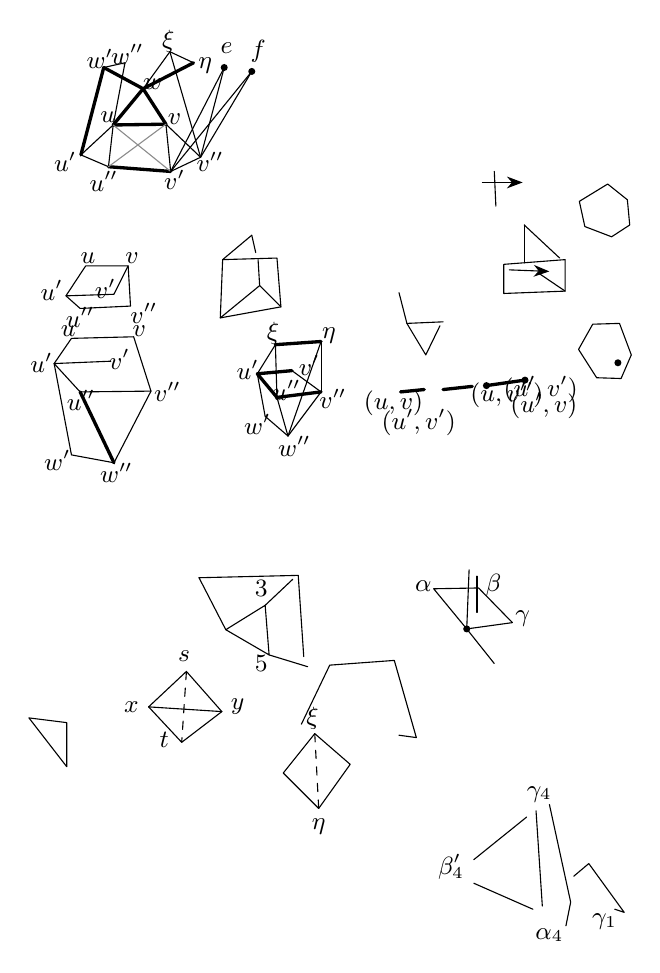
\begin{tikzpicture}[x=1mm,y=1mm,line cap=round,line join=round,font=\scriptsize]
\draw (17.6,-7.7) -- (20.3,-7.1);
\draw[very thick] (17.6,-7.7) -- (22.6,-10.4);
\draw[very thick] (17.6,-7.7) -- (14.7,-18.8);
\draw (20.3,-7.1) -- (18.8,-15);
\draw (26,-5.7) -- (22.6,-10.4);
\draw (26,-5.7) -- (29,-7.1);
\draw[very thick] (29,-7.1) -- (22.6,-10.4);
\draw (26,-5.7) -- (29.9,-19.1);
\draw[very thick] (22.6,-10.4) -- (18.8,-15);
\draw[very thick] (22.6,-10.4) -- (25.5,-14.9);
\draw[very thick] (18.8,-15) -- (25.5,-14.9);
\draw (14.7,-18.8) -- (18.8,-15);
\draw (18.8,-15) -- (18.2,-20.3);
\draw (14.7,-18.8) -- (18.2,-20.3);
\draw[very thick] (18.2,-20.3) -- (26.1,-20.9);
\draw (26.1,-20.9) -- (29.9,-19.1);
\draw (29.9,-19.1) -- (25.5,-14.9);
\draw (25.5,-14.9) -- (26.1,-20.9);
\draw[pencil] (18.2,-20.3) -- (25.5,-14.9);
\draw[pencil] (18.8,-15) -- (26.1,-20.9);
\draw (32.9,-7.7) -- (26.1,-20.9);
\draw (32.9,-7.7) -- (29.9,-19.1);
\draw (36.4,-8.2) -- (26.1,-20.9);
\draw (36.4,-8.2) -- (29.9,-19.1);
\node[pt] at (32.9,-7.7) {};
\node[pt] at (36.4,-8.2) {};
\node[inner sep=1pt] at (33.2,-5.2) {\small $e$};
\node[inner sep=1pt] at (37.2,-5.6) {\small $f$};
\node[inner sep=1pt] at (17.1,-6.6) {\small $w'$};
\node[inner sep=1pt] at (20.6,-6) {\small $w''$};
\node[inner sep=1pt] at (25.8,-4.4) {\small $\xi$};
\node[inner sep=1pt] at (30.5,-7.4) {\small $\eta$};
\node[inner sep=1pt] at (23.8,-9.8) {\small $w$};
\node[inner sep=1pt] at (18.1,-14) {\small $u$};
\node[inner sep=1pt] at (26.6,-14.3) {\small $v$};
\node[inner sep=1pt] at (12.7,-19.7) {\small $u'$};
\node[inner sep=1pt] at (31.1,-19.7) {\small $v''$};
\node[inner sep=1pt] at (17.6,-22.2) {\small $u''$};
\node[inner sep=1pt] at (26.6,-22) {\small $v'$};
\draw (15.3,-32.9) -- (20.7,-32.9) -- (21,-38) -- (14.6,-38.3) -- (12.8,-36.7) -- (15.3,-32.9);
\draw (12.8,-36.7) -- (18.9,-36.5) -- (20.7,-32.9);
\node[inner sep=1pt] at (15.6,-31.9) {\small $u$};
\node[inner sep=1pt] at (21.2,-31.9) {\small $v$};
\node[inner sep=1pt] at (11,-36) {\small $u'$};
\node[inner sep=1pt] at (17.8,-35.8) {\small $v'$};
\node[inner sep=1pt] at (14.6,-39.4) {\small $u''$};
\node[inner sep=1pt] at (22.7,-38.9) {\small $v''$};
\draw (13.5,-42.1) -- (21.4,-41.9) -- (23.6,-48.8) -- (14.6,-48.9) -- (11.3,-45.3) -- (13.5,-42.1);
\draw (11.3,-45.3) -- (18.5,-45);
\draw (11.3,-45.3) -- (13.5,-56.9) -- (18.9,-57.9) -- (23.6,-48.8);
\draw[very thick] (14.6,-48.9) -- (18.9,-57.9);
\node[inner sep=1pt] at (13.1,-41.2) {\small $u$};
\node[inner sep=1pt] at (22.1,-41.2) {\small $v$};
\node[inner sep=1pt] at (9.7,-45.2) {\small $u'$};
\node[inner sep=1pt] at (19.6,-44.8) {\small $v'$};
\node[inner sep=1pt] at (14.7,-50) {\small $u''$};
\node[inner sep=1pt] at (25.7,-48.9) {\small $v''$};
\node[inner sep=1pt] at (11.7,-57.6) {\small $w'$};
\node[inner sep=1pt] at (19.2,-59.2) {\small $w''$};
\draw (32.7,-32.1) -- (36.4,-29);
\draw (36.4,-29) -- (36.9,-31.2);
\draw (32.7,-32.1) -- (39.6,-31.9) -- (40.1,-38.1) -- (32.4,-39.5) -- (32.7,-32.1);
\draw (32.4,-39.5) -- (37.4,-35.4) -- (40.1,-38.1);
\draw (37.4,-35.4) -- (37.2,-32.1);
\draw[very thick] (39.4,-42.9) -- (45.2,-42.5);
\draw (39.4,-42.9) -- (39.6,-49.6);
\draw (45.2,-42.5) -- (45.2,-48.9);
\draw (45.2,-42.5) -- (41,-54.5);
\draw[very thick] (37.1,-46.6) -- (41.5,-46.2);
\draw (37.1,-46.6) -- (39.4,-42.9);
\draw[very thick] (37.1,-46.6) -- (39.6,-49.6);
\draw (37.1,-46.6) -- (38.1,-52);
\draw[very thick] (39.6,-49.6) -- (45.2,-48.9);
\draw (38.1,-52) -- (41,-54.5);
\draw (39.6,-49.6) -- (41,-54.5);
\draw (41.5,-46.2) -- (45.2,-48.9);
\draw (45.2,-48.9) -- (41,-54.5);
\node[inner sep=1pt] at (39.1,-41.5) {\small $\xi$};
\node[inner sep=1pt] at (46.2,-41.8) {\small $\eta$};
\node[inner sep=1pt] at (35.9,-46.1) {\small $u'$};
\node[inner sep=1pt] at (43.7,-45.5) {\small $v'$};
\node[inner sep=1pt] at (40.8,-48.7) {\small $u''$};
\node[inner sep=1pt] at (46.7,-49.8) {\small $v''$};
\node[inner sep=1pt] at (37.1,-53) {\small $w'$};
\node[inner sep=1pt] at (41.8,-55.8) {\small $w''$};
\draw (55.1,-36.3) -- (56.1,-40.2) -- (58.5,-44.2) -- (60.3,-40.5);
\draw (56.1,-40.2) -- (60.7,-40);
\draw[very thick] (55.3,-48.9) -- (58.3,-48.6);
\node[inner sep=1pt] at (54.4,-50.3) {\small $(u,v)$};
\node[inner sep=1pt] at (57.6,-52.8) {\small $(u',v')$};
\draw[-{Stealth[length=2mm]}] (65.7,-22.3) -- (70.8,-22.3);
\draw (67.2,-20.9) -- (67.4,-25.3);
\draw (78,-24.7) -- (81.6,-22.5) -- (84.1,-24.5) -- (84.4,-27.7) -- (82.1,-29.2) -- (78.7,-27.9) -- cycle;
\draw (68.4,-32.7) -- (76.2,-32.1) -- (76.2,-36.1) -- (68.4,-36.4) -- cycle;
\draw (71,-27.7) -- (71,-32.5);
\draw (71,-27.7) -- (75.5,-31.9);
\draw[-{Stealth[length=2mm]}] (69.1,-33.4) -- (74.2,-33.6);
\draw (72.8,-33.8) -- (76.2,-36.1);
\draw (79.7,-40.3) -- (83.1,-40.2) -- (84.6,-44.2) -- (83.3,-47.2) -- (80.2,-47.1) -- (77.9,-43.5) -- cycle;
\node[pt] at (82.9,-45.2) {};
\draw[very thick] (60.7,-48.6) -- (64.4,-48.2);
\draw[very thick] (66.2,-48.1) -- (71.1,-47.4);
\node[pt] at (66.2,-48.1) {};
\node[pt] at (71.1,-47.4) {};
\node[inner sep=1pt] at (68.8,-49.3) {\small $(u,v'')$};
\node[inner sep=1pt] at (73.1,-48.6) {\small $(u',v')$};
\node[inner sep=1pt] at (73.5,-50.6) {\small $(u',v)$};
\draw (8.1,-90.3) -- (12.9,-90.9) -- (12.9,-96.5) -- cycle;
\draw (23.3,-88.9) -- (28.1,-84.4) -- (32.6,-89.5) -- (27.5,-93.4) -- cycle;
\draw (23.3,-88.9) -- (32.6,-89.5);
\draw[dashed] (28.1,-84.4) -- (27.5,-93.4);
\node[inner sep=1pt] at (27.8,-82.4) {\small $s$};
\node[inner sep=1pt] at (21.1,-88.9) {\small $x$};
\node[inner sep=1pt] at (34.6,-88.9) {\small $y$};
\node[inner sep=1pt] at (25.3,-93.1) {\small $t$};
\draw (44.4,-92.3) -- (40.4,-97.3) -- (44.9,-101.8) -- (48.9,-96.2) -- cycle;
\draw[dashed] (44.4,-92.3) -- (44.9,-101.8);
\node[inner sep=1pt] at (44.1,-90.3) {\small $\xi$};
\node[inner sep=1pt] at (44.9,-104.1) {\small $\eta$};
\draw (42.7,-91.1) -- (46.3,-83.6) -- (54.5,-83) -- (57.3,-92.8) -- (55.1,-92.5);
\draw (59.5,-73.9) -- (65.2,-73.8) -- (69.5,-78.2) -- (63.7,-79) -- cycle;
\draw (63.7,-79) -- (67.2,-83.4);
\draw (64,-71.5) -- (63.7,-79);
\draw (65,-72.3) -- (65,-76.9);
\node[pt] at (63.7,-79) {};
\node[inner sep=1pt] at (58.2,-73.6) {\small $\alpha$};
\node[inner sep=1pt] at (67.1,-73.4) {\small $\beta$};
\node[inner sep=1pt] at (70.8,-77.7) {\small $\gamma$};
\draw (72.5,-102.1) -- (73.3,-114.2);
\draw (74.2,-101.3) -- (76.9,-113.7) -- (76.3,-116.7);
\draw (64.6,-108.3) -- (71.3,-102.9);
\draw (64.6,-111.3) -- (72.1,-114.6);
\draw (77.3,-110.4) -- (79.2,-108.8) -- (83.7,-115) -- (82.5,-114.6);
\node[inner sep=1pt] at (72.9,-100) {\small $\gamma_4$};
\node[inner sep=1pt] at (61.7,-109.2) {\small $\beta'_4$};
\node[inner sep=1pt] at (74.2,-117.9) {\small $\alpha_4$};
\node[inner sep=1pt] at (81.2,-116.2) {\small $\gamma_1$};
\draw (29.7,-72.5) -- (42.3,-72.2);
\draw (29.7,-72.5) -- (33.1,-79.1);
\draw (42.3,-72.2) -- (43,-82.5);
\draw (33.1,-79.1) -- (38.1,-76) -- (38.6,-82.3) -- cycle;
\draw (38.1,-76) -- (41.6,-72.7);
\draw (38.6,-82.3) -- (43.5,-83.8);
\node[inner sep=1pt] at (37.6,-73.9) {\small $3$};
\node[inner sep=1pt] at (37.6,-83.4) {\small $5$};
\end{tikzpicture}
\end{document}
